\chapter{Full Pairwise Connectivity With Spatial Coherence}
\label{chap:method1}

% the functional activity has the multiple comparision problem. 
In this chapter, we present a new method for spatial regularization of
functional connectivity maps based on MRF priors. The high level of noise in
fMRI leads to errors in functional connectivity detection algorithms. A common
approach to mitigate the effects of noise is to apply spatial Gaussian
smoothing, which can lead to blurring of regions beyond their actual boundaries
and the loss of small connectivity regions. Recent work has suggested MRF as an
alternative spatial regularization in the detection of fMRI activation in
task-based paradigms. We propose to apply MRF priors to the computation of
functional connectivity in resting-state fMRI. Our Markov priors are in the
space of pairwise voxel connections, rather than in the original image space,
resulting in a MRF whose dimension is twice that of the original image. The high
dimensionality of the MRF estimation problem leads to computational
challenges. We present an efficient, highly parallelized algorithm on the
graphics processing unit (GPU). We validate our approach on a synthetically
generated example as well as real data from a resting state fMRI study.

\section{Motivation}
To show the noise level and the impact of spatial smoothing on the functional
connectivity estimation, we take a seed voxel at the MNI coordinate (42, 16, 25)
and compute the correlation between this seed region and every other voxel's
BOLD signal in the same volume of the spatially smoothed rs-fMRI volume, and
show the correlation map at Figure \ref{fig:conexample}. The seed signal is
computed by averaging the BOLD signal of voxels within 5 mm distance from the
seed voxel. Following  standard seed-based functional connectivity methods,
we average the BOLD signal of the voxels within r = 5 mm from the seed voxel,
and use the averaged signal as a surrogate of the BOLD signal at this
coordinate. We then compute the sample correlation between this average signal
and every other voxel's BOLD signal in the full volume. For display purposes, we
only show the correlation map of one slice where the seed region is
located. Figure \ref{fig:fmrislice} shows the first time point of the original
BOLD signal. As expected, it is impossible to see any meaningful patterns from
this image, since the functional connectivity is not represented by a voxel's
intensity at a single time point, but the average effect across all time
points. Figure \ref{fig:corrmap} shows the linear correlation map with the seed
regions, with the red dot giving the location of the seed region. We can see the
symmetric location of the seed region on the other hemisphere shows higher
intensity of correlation, suggesting these voxels are more positively correlated
with the seed. In Figure \ref{fig:corrmap_th}, we show the correlation map
thresholded at 0.3. Since the seed region belongs to the default model network
(DMN), an important component in the intrinsic functional system, we expect to
see other spatially remote regions in the same network have higher correlation
in \ref{fig:corrmap_th}, We observe one region on the same location of the
opposite hemisphere, and also one region at the prefrontal lobe remains after
thresholding. However, overall the spatial patterns are hard to identify, and there
are also some false-positive detections. One reason for the difficulty in
detecting the connectivities is the large amount of noise in the data, and the
spatial smoothing in the preprocessing step. We aim to address this problem in
this chapter.


In both task-based and rs-fMRI the impact of imaging noise can be reduced by
taking advantage of the spatial correlations between neighboring voxels in the
image. A common approach used for instance in statistical parametric mapping
(SPM)\cite{worsley_analysis_1995} is to apply a spatial Gaussian filter to
smooth the signal prior to statistical analysis. However, this can lead to
overly blurred results, where effects with small spatial extent can be lost and
detected regions may extend beyond their actual boundaries. An alternative
approach to spatial regularization that has been proposed for task activation
paradigms is to use a Markov random field (MRF) prior~\cite{ou_spatial_2005,
  descombes_spatio-temporal_1998, descombes_fmri_1998,
  woolrich_fully_2004,cosman_exact_2004}, which models the conditional
dependence of the signals in neighboring voxels.

In this chapter we propose to use MRF models in rs- fMRI to leverage spatial
correlations in functional connectivity maps. Unlike previous MRF-based
approaches, which use the neighborhood structure defined by the original image
voxel grid, the neighborhoods in functional connectivity must take into account
the possible relationships between spatially distant voxels. Therefore, we
define the neighborhood graph on the set of all voxel pairs. This results in a
Markov structure on a grid with twice the dimensions of the original image data,
i.e., the pairwise connectivities for three-dimensional images results in a
six-dimensional MRF. The neighborhood structure is defined so that two voxels
are more likely to be connected if they are connected to each other's spatial
neighbors.

We combine the Markov prior on functional connectivity maps with a likelihood
model of the time series correlations in a posterior estimation problem.
Furthermore, we  solve for the unknown parameters of the MRF and likelihood
using the EM algorithm that we discussed in Section \ref{chap:em}. In the
estimation step the posterior random field is sampled using Gibbs sampling and
estimated using mean field theory, also known as variational inference.

In the next section we describe our MRF model of functional connectivity maps.
In Section~\ref{sec:methods} we give the details of the algorithm to estimate
the functional connectivity probabilities, including implementation details for
the GPU solver. Finally, in Section~\ref{sec:results} we demonstrate the
advantages of our approach on a synthetically generated data set as well as on
real rs-fMRI data.

\section{Methods}
\label{sec:methods}
Our framework for functional connectivity is a Bayesian approach in which we
estimate the posterior distribution of the connectivity between voxels,
conditioned on the fMRI data. Let $X = \{x_{ij}\}$ denote the functional
connectivity map, i.e., a map denoting whether each pair of voxels $i,j$ is
connected, and let $Y$ denote the original fMRI data, or some measurement
derived from the fMRI. In this work we take $Y$ to be the map of correlations
between pairs voxel time series. The posterior distribution is then
proportionally given by
\begin{equation}
\label{eq:posterior}
P(X \, | \, Y) \prop P(X) \cdot P(Y \, | \, X).
\end{equation}
In this work we model $P(X)$, the prior on the connectivity map, using a
MRF, and the likelihood $P(Y \, | \, X)$ using Gaussian models of the
Fisher transformed correlation values. We now give details for both of these
pieces of the model.


\subsection{Markov prior}
Conventional image analysis applications of MRFs~\cite{li_markov_2009} define
the set of sites of the random field as the image voxels, with the neighborhood
structure given by a regular lattice. Because we are studying the pairwise
connectivity between voxels, we need to define a MRF in the higher-dimensional
space of voxel location pairs. Thus, if $\Omega \subset \mathbb{Z}^d$ is a
$d$-dimensional image domain, then the sites for our connectivity MRF form the
set $\mathcal{S} = \Omega \times \Omega$. Let $i, j \in \Omega$ be voxel
locations, and let $\mathcal{N}_i, \mathcal{N}_j$ denote the set of neighbors of
voxel $i$ and $j$, respectively, in the original image lattice. Then the set of
neighbors for the site $(i, j) \in \mathcal{S}$ is given by $\mathcal{N}_{ij} =
(\{i\} \times \mathcal{N}_j) \cup (\mathcal{N}_i \times \{j\})$. In other words,
two sites are neighbors if they share one coordinate and their other coordinates
are neighbors in the original image lattice. This neighborhood structure will
give us the property in the MRF that two voxels $i, j$ in the image are more
likely to be connected if $i$ is connected to $j$'s neighbors or
vice-versa. Equipped with this graph structure, $\mathcal{S}$ is a regular
$2d$-dimensional lattice. With the node set $\cX$ and neighboring system $\cN$,
we define a graph $\cG$ that we call the {\em connectivity graph}. Figure
\ref{fig:6dmrf} gives an illustration of how this connectivity graph is defined.

We next define a multivariate random variable $X = \{ x_{ij} \}$ on the set
$\mathcal{S}$, where each $x_{ij}$ is a binary random variable that
denotes the connectivity ($x_{ij} = 1$) or lack of connectivity ($x_{ij} = -1$)
between voxel $i$ and $j$. If $A \subset \mathcal{S}$, let $X_A$ denote the
set of all $x_{ij}$ with $(i,j) \in A$, and let $X_{-ij}$ denote the
collection of all variables in $X$ excluding $x_{ij}$. For $X$ to be a
MRF it must satisfy
\begin{equation*}
  P( x_{ij} \, | \, X_{-ij}) = p(x_{ij} \, | \, x_{\mathcal{N}_{ij}}).
\end{equation*}
According to the Hammersley and Clifford theorem~\cite{besag_spatial_1974}, $X$
is a Markov random field if and only if it is also a Gibbs distribution, defined
as
\begin{equation}
  P(X) = \frac{1}{Z}\exp\left(-U(X)\right), 
\end{equation}
where $U$ is the energy function $U(X) = \sum_{c \in \mathcal{C}}
V_c$, with potentials $V_c$ defined for each clique $c$ in the clique
set $\mathcal{C}$. The partition function $Z = \sum_{X} \exp(-U(X))$
is a normalizing constant, where the summation is over all possible
configurations of $X$. We use a particular form of MRF---the
Ising model---a commonly used model for MRFs with binary states. In
this model the energy function is given by
\begin{equation}
U(X) = - \beta \sum_{( ij, mn )} x_{ij} x_{mn},
 \label{eq:A1}
\end{equation}
where the summation is over all edges $( ij, mn )$ on the graph $\cG$, i.e., all
adjacent voxel pairs $(i,j), (m,n)$ in the connectivity graph. When $\beta > 0$,
this definition favors similarity of neighbors. An alternative definition is to
make the MRF prior also contain the data term, such as the strength of the
connection between neighboring nodes also depends on the data. Where the
observed correlation value of two nodes are different, the strength of the MRF
prior will be decreased. This is the conditional random field we have discussed
in Section \ref{sec:crf}.
\subsection{Likelihood model}
We now define the likelihood model, $P(Y \, | \, X)$, which connects the
observed data $Y$ to our MRF. Because we are interested in the functional
connectivity between pairs of voxels, we compute the correlation between the
time courses of each pair of voxels, and get a correlation matrix $Y =
\{y_{ij}\}$. Just as in the case of the random field $X$, the correlation matrix
$Y$ is also defined on the $2d$-dimensional lattice $\mathcal{S}$. Linear
correlation is not the only choice for $Y$. We can use any statistic, as long as
it indicates the affinity between two voxel time series. Another possibility
could be frequency domain measures, such as the
coherence~\cite{mller_multivariate_2001}, although the definition of likelihood
function is not straightforward for such similarity measurement. On the other
hand, simple linear correlation has the advantage that after the Fisher
transformation, the correlation statistics have a well defined distribution. If
the original variables $y_i$ and $y_j$'s intensities across all time points are
Gaussian, then the sample correlation estimated from the intensities are also
Gaussian after Fisher transformation. Therefore, the conditional distribution of
$P(y_{ij} | x_{ij})$ is a well-defined Gaussian distribution.

Before defining the full data likelihood, we start with a definition of the {\em
  emission function} at a single site $s_{ij} \in \mathcal{S}$. This is defined
as the conditional likelihood, $P(y_{ij} \, | \, x_{ij})$, and is interpreted as
the probability of the observed correlation, given the state of the connectivity
between voxels $i$ and $j$. We model the emission function as a Gaussian
distribution with unknown mean and variance on the Fisher transformed
correlation $y_{ij}$, that is,
\begin{equation}
\label{eq:emission}
P(y_{ij} \,|\, x_{ij} = k) = \frac{1}{\sqrt{2\pi} \sigma_k} \exp \left( -\frac{(F(y_{ij}) -  \mu_k)^2}{2\sigma_k^2}\right),
\end{equation}
where $F$ denotes the Fisher transform. Notice that each correlation $y_{ij}$ on
site $s_{ij}$ only depends on the latent variable $x_{ij}$ on the same site, and
does not depend on neighbors of $x_{ij}$. Alternative definitions exist. For
example, the observed correlation data $y_{ij}$ can also depend on the
neighbors of $x_{ij}$, similar to the work of Geman et
al.~\cite{geman1984stochastic}. This is equivalent to adding more edges on the
graphical model, and therefore the posterior inference will be more
complicated. In this work, we use a simple model that has a one-to-one
correspondence between $x_{ij}$ and $y_{ij}$. Given the above setting, the full
likelihood is given by
\begin{equation}
\label{eq:likelihood}
P(Y \, | \, X) = \prod_{s_{ij}\in\mathcal{S}} P(y_{ij} \, | \, x_{ij}).
\end{equation}

\section{Estimation via expectation maximization}
\label{sec:algorithm}
Having defined the data likelihood and MRF prior in the previous section, we are
now ready to describe the maximization of the posterior given
by~\eqref{eq:posterior}. For this we need to determine the model parameters,
$\beta$ in \eqref{eq:A1} and $(\mu_k, \sigma_k^2)$ in
\eqref{eq:emission}. Rather than arbitrarily setting these parameters, we
estimate them using the EM algorithm. Exact
computation of the full posterior~\eqref{eq:posterior} is intractable, due to
the combinatorial number of terms in the partition function $Z$. Therefore, we
instead maximize the approximate posterior given by the pseudo-likelihood
function~\cite{li_markov_2009,besag_spatial_1974},
\begin{equation}
PL(X, Y) = \prod_{ij}^{}P (x_{ij}|x_{\mathcal{N}_{ij}}) P(y_{ij}|x_{ij}). \label{eq:2}
\end{equation}

In the E-step, the parameters are held fixed and we compute the posterior
probability for each $x_{ij}$, and sample $x_{ij}$ from the posterior
distribution using Gibbs sampling. We then compute the expected value of each
connectivity node by mean field theory. After we compute the posterior of
current point $x_{ij}$, we update $x_{ij}$ with its expected value $\langle
x_{ij} \rangle$. The equivalence of posterior probability and the expectation of
binary random variable is discussed in Section \ref{chap:mathvar}.

In the M-step, the complete data $\{\langle X\rangle, Y\}$ are available, and the
parameters can be estimated by maximizing the joint pseudo-likelihood given
by~\eqref{eq:2} using Newton's method. After several iterations of this EM
algorithm, we get parameters as our MAP estimates. During parameter estimation,
the joint likelihood can be factorized into two separate terms of the prior and
the conditional likelihood, and the parameter $\beta$ can be estimated by
maximizing the MRF prior (equivalently the pseudo-likelihood) by Newton's
method. The estimation of $\mu$ and $\sigma^2$ can be done in closed from just
like the standard Gaussian mixture model, as shown in Section \ref{sec:parest}.

\subsection{GPU implementation}
 The whole algorithm involves updating a high dimensional connectivity matrix
 $X$ iteratively, and hence it has high computation cost. We designed a parallel
 Markov random field updating strategy on a graphics processing unit (GPU). The
 algorithm takes only a few minutes compared with more than 1 hour on the CPU
 counterpart.


To fit the algorithm into GPU's architecture, we use some custom
strategies. First, because GPU only support three-dimensional array, we need to
reshape $X$ and $Y$ defined originally on a higher dimensional graph by linear
indexing their original subscripts. This is especially difficult for brain fMRI
data because the gray matter voxels reside in an irregular three-dimensional lattice. Specific
data structures are used for mapping between original voxel subscripts and their
linear index $i$ and $j$. Second, to update each site of the MRF in parallel, we
have to make sure a site is not updated simultaneously with its neighbors,
otherwise the field tends to be stuck in a checkerboard-like local maximum, as
indicated by Figure \ref{fig:checkerboard}.  Our strategy is to divide all the
sites of the field into several subgroups, such that a site is not in the same
subgroup with its neighbors.  We then can update the subgroup sequentially,
while the data in subgroups are updated simultaneously. The whole procedure is
summarized in Algorithm \ref{alg:1}.


\begin{algorithm}[p]
  \caption{MAP estimation by EM}
  \label{alg:1}
  \begin{algorithmic}
    \REQUIRE Sample correlation matrix $\mat Y$.
    \STATE Init posterior matrix by maximizing conditional likelihood
    $P(y_{ij}|x_{ij})$.  
    \WHILE{$\Delta \{\beta, \mu, \sigma^2 \} >
      \varepsilon$ } 
    \STATE \textbf{E step: }

    (a) Based on the current
    parameters, compute the posterior by \eqref{eq:2}.

    (b) Repeatedly Do Gibbs Sampling until the field  stabilizes.

    (c) Based on current value of $x_{ij}$, iteratively compute the mean
    field for all nodes in $\mathcal{S}$ until the field is stable.

    \STATE \textbf{M step: } 

    (d) With complete data $\{\mat X, \mat
    Y\}$, estimate $\beta$ , $\mu$ and $\sigma^2$ by maximizing
    \eqref{eq:2}.
    \ENDWHILE
    \RETURN posterior matrix $\mat X$.
  \end{algorithmic}
\end{algorithm}

It is noted this updating scheme is closely related to the coding method of
parameter estimation of MRF that we discussed in Section \ref{sec:parest}. Both
approaches split the variables into multiple subgroups. They differ in that
for coding methods, the separation is used to get independent variables within
the subgroup, while here the voxels in subgroups are independent so we can
update them in parallel.


\section{Results}
\label{sec:results}
In this section, we give the experimental results for both  simulated data and
real fMRI data. We compare the results of various methods on simulated data
with the ground truth to show the proposed method's performance. In the real
data experiment, we compare the results with the functional connectivity map of
other literatures.


\subsection{Synthetic data} 
\label{sec:m1syn}
We first construct a synthetic data set consisting of a $100\times 1$
one-dimensional image, with each pixel a 300-point time course signal. The
one-dimensional image will guarantee the connectivity map be in
two-dimensional space and can be visualized easily. The time course was
constructed with a baseline DC signal of 800, plus additive Gaussian noise of
zero mean and variance 50. We then added a sine wave signal of frequency 0.2
and amplitude 20 to two distant regions of the image. The goal is to detect
the connectivity between these two distant regions. The true connectivity
value will be one between those pixels containing the sine wave signal,
otherwise it is defined as $-1$ for lack of connectivity between signal and
noise, and between noise time series. The true connectivity map is shown in
Figure~\ref{fig:6dconn1}.

To compare our MRF model with conventional Gaussian blurring of the correlation
map, we applied both approaches to the synthetic data (Figure
~\ref{fig:6dconn}). On the correlation map in the top row, we see smoothing does
remove noise and results in a correlation map that looks more like the true
connectivity map. However, it also creates several errors, most noticeably false
positives around the diagonal (Figure~\ref{fig:6dconn5}). This is because
without prior knowledge of the scale of the patterns we are interested in, the
choice of smoothing kernel size is arbitrary. Therefore, a large kernel size
will enforce the signals of many voxels to look similar, and the following correlation
map will have more false-positive detections. Figure~\ref{fig:6dconn6} shows the
proposed MRF method better detects the true connectivity regions while removing
most false positives.
 

\subsection{Resting-state fMRI} 
Next we tested our method on real data from healthy control subjects in a
resting-state fMRI study. BOLD EPI images (TR= 2.0 s, TE = 28 ms, GRAPPA
acceleration factor = 2, 40 slices at 3 mm slice thickness, 64 x 64 matrix, 240
volumes) were acquired on a Siemens 3 Tesla Trio scanner with 12-channel head
coil during the resting state, eyes open. The data was motion corrected by SPM
software and registered to a T2 structural image. We used a gray matter mask
from an SPM tissue segmentation so that only gray matter voxels are counted in
the connectivity analysis. We do \emph{not} spatially smooth the data, in order
to see the benefit of replacing spatial smoothing with our MRF method. Before
computing the correlations, the time series at all voxels are linearly detrended
by least squares regression.

Figure \ref{fig:invivo1} compares the real data results using no spatial
regularization, Gaussian smoothing, and the proposed MRF model. Though the
posterior connectivity of the MRF is computed between every pair of voxels
within a slice, for visualization purposes, only the posterior of the
connectivity between one voxel and the slice is shown. We chose to visualize
the connectivity to a voxel in the posterior cingulate cortex (PCC) because
this is known to be involved in the default mode
network~\cite{raichle2001default}, with connections to the medial prefrontal
cortex (MPFC). The results show that Gaussian smoothing is able to remove
noise, but is unable to find a clear connection between the PCC and the
MPFC. Our proposed MRF model (\ref{fig:invivo13} and \ref{fig:invivo16}) is
able to remove spurious connections, and also clearly shows a connection to
the MPFC.

To show the strongest connections found by each method, Figure
\ref{fig:invivo2} shows the thresholded connectivity maps overlaid on T2
structural image. Images in the first two columns are thresholded such that
the top $5\%$ voxel correlations are shown. For the MRF in \ref{fig:invivo23}
and \ref{fig:invivo26}, the MAP estimate is shown.


\section{Discussion}
Functional connectivity is a key step of understanding the human brain's
functional networks, since it contains all the information of how each
functional region interacts with other regions. There are multiple ways of
modeling functional systems. One is defining some regions of interest (ROI) as
the nodes on the graph, and estimate the connectivities among these ROIs. The
ROI definition has no standard to follow. One can either define them according
to the anatomical structure, or by a parcellation on the functional data. The
other way of representing functional networks is to cluster the full brain
volume (indeed the gray matter voxels) into small regions. Regions in the same
cluster are highly connected even if they are spatially remote. Our method
outputs a posterior matrix that includes all the connectivity information between
each pair of voxels. One potential usage of the full connectivity matrix is 
exploring the connectivity given a single seed coordinate. That is, given the
seed, one can explore the posterior connectivity between the seed voxel and the
full brain volume in real time. Such full connectivity will be dynamically
shown with the changing seed's location. Such a dynamic, and potentially
user-interactive functional connectivity exploratory concept has been partly
realized by Yeo et al.~\cite{yeo2011organization}, though they did not use MRF
to model the spatial constraints of the connectivity variables. Instead, Yeo
et al. use
a large group of subjects and obtained a highly consistent population functoinal
connectivity network. The network can be visualized given a seed region and also
the change of the network patterns when the seed changes.

On the optimization side, the MCEM algorithm, and the wider class of sampling
methods are potentially good candidates for the application of GPU. Although
theoretically the computation on GPU needs independence between the data
points, the order of voxels being sampled have no effect on the quality of the
samples once the sampling reaches stationary distribution. Therefore, even at
each scan, the order, or the schedule of the data points change in an
undetermined way within the GPU cores, we can still get samples in the target
distribution give enough burn-in time. Alternative optimization methods other
than MCEM exist, such as graph cut. However, in our experiments with graph
cuts, we found the local finer patterns are sometimes ignored by graph
cut. The estimated hidden variables are accordingly mostly blob-like patterns
with small boundary-area ratio. So graph cut optimization is more suitable for
the recognition of blob-like patterns. Such preference does not necessarily
reflect the true structure in our fMRI data. As a result, the estimation of
the parameters $\beta$ in \eqref{eq:A1} is also biased towards a larger value
than the true value, since the true $X$ is not as smooth as the estimated
one. Therefore, we choose to use MCEM in our EM procedure for unbiased
estimation of parameters.

One weakness of the pairwise connectivity estimation routine is lack of
visualization for all the functional networks as spatial maps. Only when the
input image is one-dimensional, such as the synthetic data example we used in
Section \ref{sec:m1syn}, can the connectivity map be visualized on a
two-dimensional plane. In general three-dimensional volume image as input, the
connectivity matrix is in a six-dimensional space and cannot be shown in a
straightforward way. Once the posterior connectivity matrix is computed, we
still need to give a seed region in order to map all the functional systems
that are connected to the seed. We will discuss methods of estimating multiple
functional networks and show them in a single volume image in the next
chapter.



\begin{figure}[p]
  \centering
  \begin{subfigure}[b]{0.3\textwidth}
    \centering
    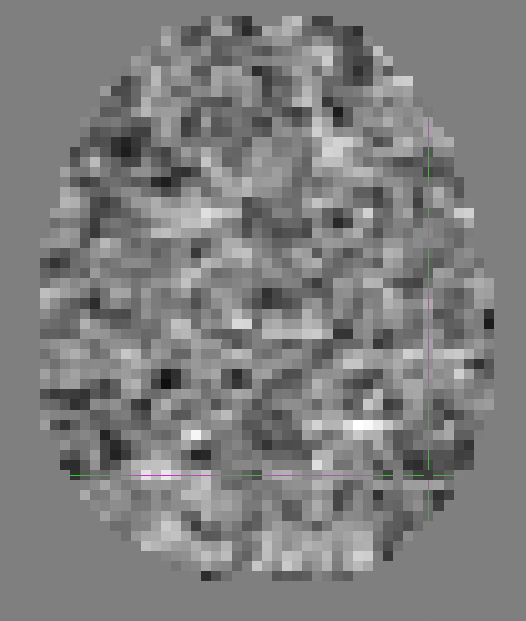
\includegraphics[height=\textwidth]{figures/method1/fmrislice}
    \caption{One slice of a resting-state fMRI dataset at $z = 25$. }
    \label{fig:fmrislice}
    \end{subfigure}
~
  \begin{subfigure}[b]{0.3\textwidth}
    \centering
    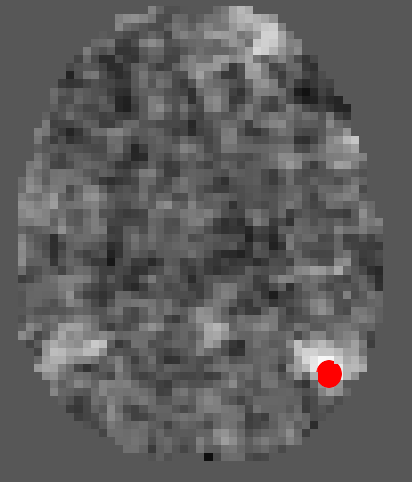
\includegraphics[height=\textwidth]{figures/method1/corrmap}
    % x = 42, y = 16, z = 25
    \caption{Correlation map between a seed and the current slice.}
    \label{fig:corrmap}
    \end{subfigure}
~
  \begin{subfigure}[b]{0.3\textwidth}
    \centering
    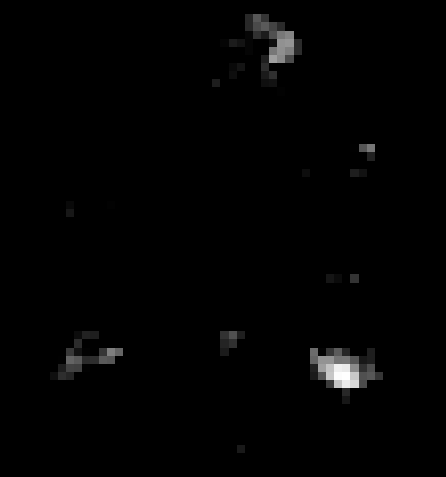
\includegraphics[height=\textwidth]{figures/method1/corrmap_th}
    \caption{The correlation map thresholded at 0.3.}
    \label{fig:corrmap_th}
    \end{subfigure}
  \caption{An example of correlation map with a seed in the default model
    network on the rs-fMRI data set.}
  \label{fig:conexample}
\end{figure}

\begin{figure}[p]
  \centering
  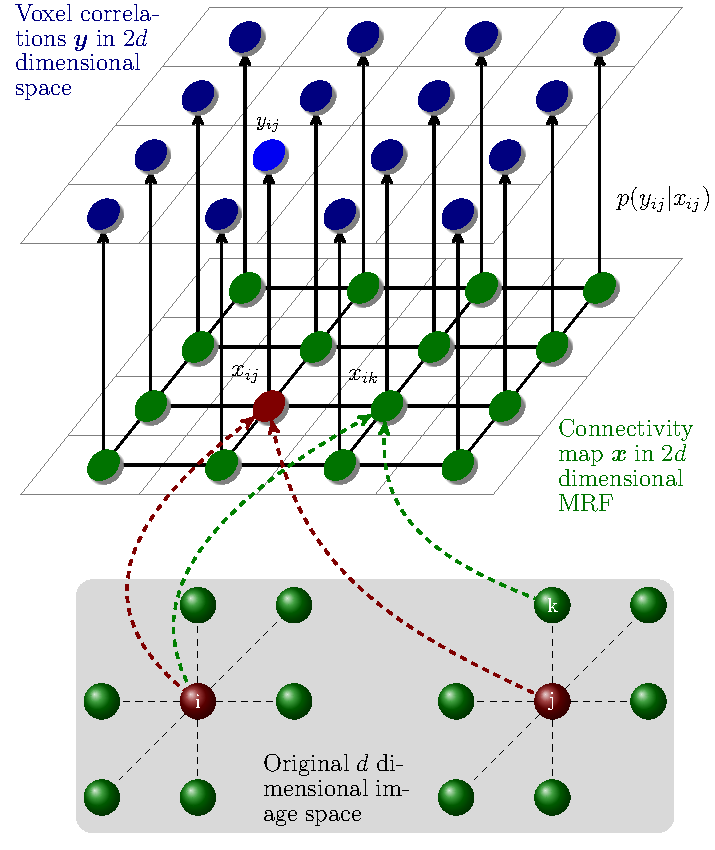
\includegraphics[width=0.5\textwidth]{figures/method1/6dmrf}
  \caption{MRF prior of the connectivity variables. Each node of the graph
    represents a pairwise connectivity variable between voxel $i$ and $j$. An
    edge is added between two nodes $x_{ij}$ and $x_{ik}$ if $k$ is the neighbor
    of voxel $j$. The graph where the MRF is defined is twice the dimensions
    of the original image domain, i.e., six dimensions. Given the hidden variable
    $X$, the observed sample correlation values are assumed to be generated
    from a Gaussian distribution with unknown parameter $\cN(y_{ij} | x_{ij}; \mu,
    \sigma^2)$. }
  \label{fig:6dmrf}
\end{figure}

\begin{figure}[p]
  \centering
  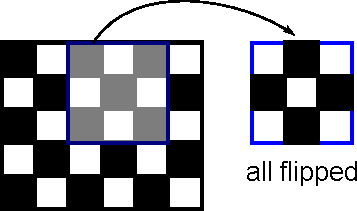
\includegraphics[width=0.5\textwidth]{figures/method1/checkerboard}
  \caption{Ideally the update of each voxel is independent of other voxels in
    order to be used on the GPU. In our Gibbs sampling, although the sampling of
    each voxel depends on its neighbors, the order of the voxels being updated
    does not matter. Upon convergence, the image will be a sample of the target
    Gibbs distribution. However, numerically, the sampling tends to be stuck in
    this local minimum of checkerboard image. At the current state, each voxel has a
    neighbor with a different state, and the sampling flips the color
    of all voxels in the next stage.}
  \label{fig:checkerboard}
\end{figure}

\begin{figure}[p] 
  \centering 
  \begin{subfigure}[t]{0.3\textwidth}
    \centering
    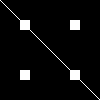
\includegraphics[width=\textwidth]{figures/method1/newtoy/trueConn}
    \caption{ground-truth connectivity}
    \label{fig:6dconn1}
    \end{subfigure}
~
  \begin{subfigure}[t]{0.3\textwidth}
    \centering
    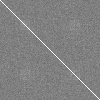
\includegraphics[width=\textwidth]{figures/method1/newtoy/corrNoSmooth}
    \caption{ correlation of original, noisy data.}
    \label{fig:6dconn2}
    \end{subfigure}
~
  \begin{subfigure}[t]{0.3\textwidth}
    \centering
    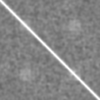
\includegraphics[width=\textwidth]{figures/method1/newtoy/SampleCorr}
    \caption{correlation of Gaussian-smoothed data.}
    \label{fig:6dconn3}
    \end{subfigure}

  \begin{subfigure}[t]{0.3\textwidth}
    \centering
    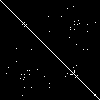
\includegraphics[width=\textwidth]{figures/method1/newtoy/threholdCorrRaw}
    \caption{connectivity based on noisy correlations.}
    \label{fig:6dconn4}
    \end{subfigure}
~
  \begin{subfigure}[t]{0.3\textwidth}
    \centering
    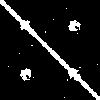
\includegraphics[width=\textwidth]{figures/method1/newtoy/threholdCorrSmoothed}
    \caption{connectivity based on smoothed data.}
    \label{fig:6dconn5}
    \end{subfigure}
~
  \begin{subfigure}[t]{0.3\textwidth}
    \centering
    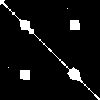
\includegraphics[width=\textwidth]{figures/method1/newtoy/newpost_sym2}
    \caption{connectivity computed using proposed MRF model}
    \label{fig:6dconn6}
    \end{subfigure}

    \caption[Test on synthetic data.]{Test of synthetic data by using
      correlation and MRF method proposed in this work. (a) Ground truth
      connectivity map. (b) Connectivity based on smoothed data. (c)
      Correlation of Gaussian-smoothed data. (d) Connectivity based on noisy
      correlations. (e) Connectivity based on smoothed data. (f) Connectivity
      computed using proposed MRF model. }
  \label{fig:6dconn}
\end{figure}


\begin{figure}[p] 
  \centering 
  \begin{subfigure}[t]{0.3\textwidth}
    \centering
    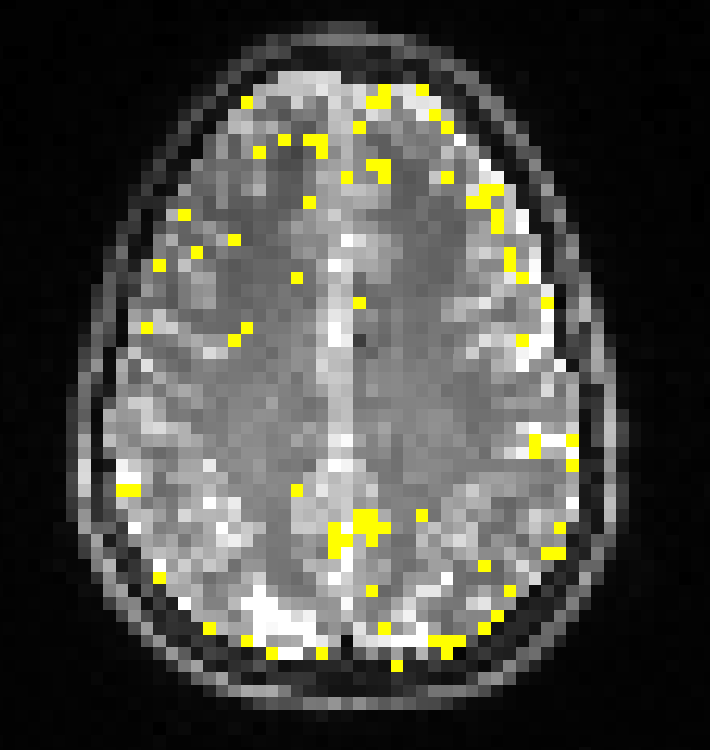
\includegraphics[width=\textwidth]{figures/method1/invivo1/r1}
    \caption{Sub1: correlation map without smoothing.}
    \label{fig:invivo11}
    \end{subfigure}
~
  \begin{subfigure}[t]{0.3\textwidth}
    \centering
    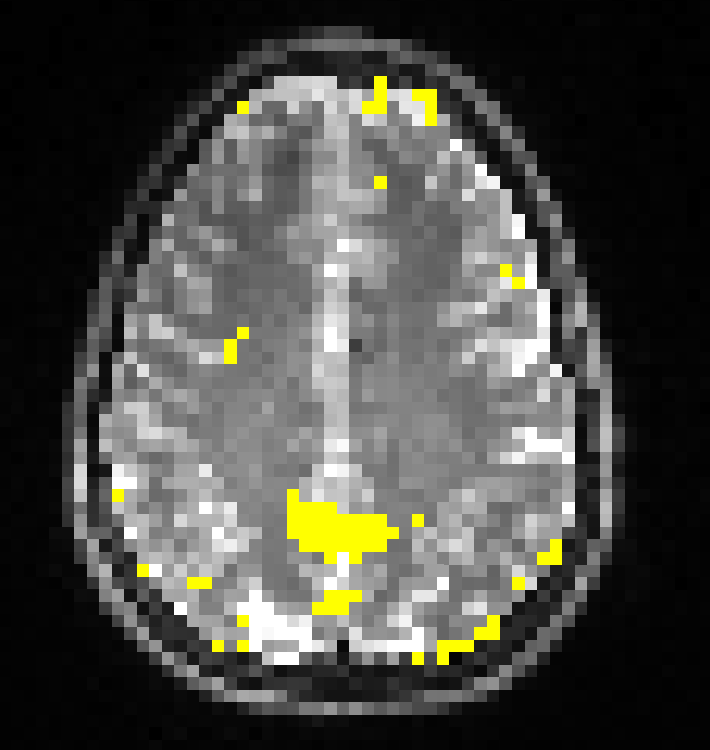
\includegraphics[width=\textwidth]{figures/method1/invivo1/r1_smooth}
    \caption{Sub1: correlation map with smoothing.}
    \label{fig:invivo12}
    \end{subfigure}
~
  \begin{subfigure}[t]{0.3\textwidth}
    \centering
    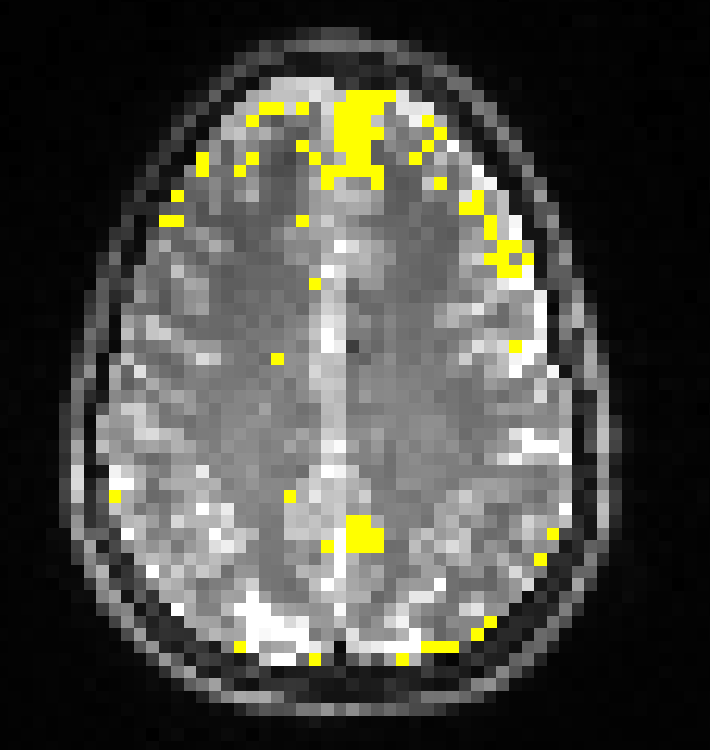
\includegraphics[width=\textwidth]{figures/method1/invivo1/r1_mrf}
    \caption{Sub1: posterior probability by MRF.}
    \label{fig:invivo13}
    \end{subfigure}

  \begin{subfigure}[t]{0.3\textwidth}
    \centering
    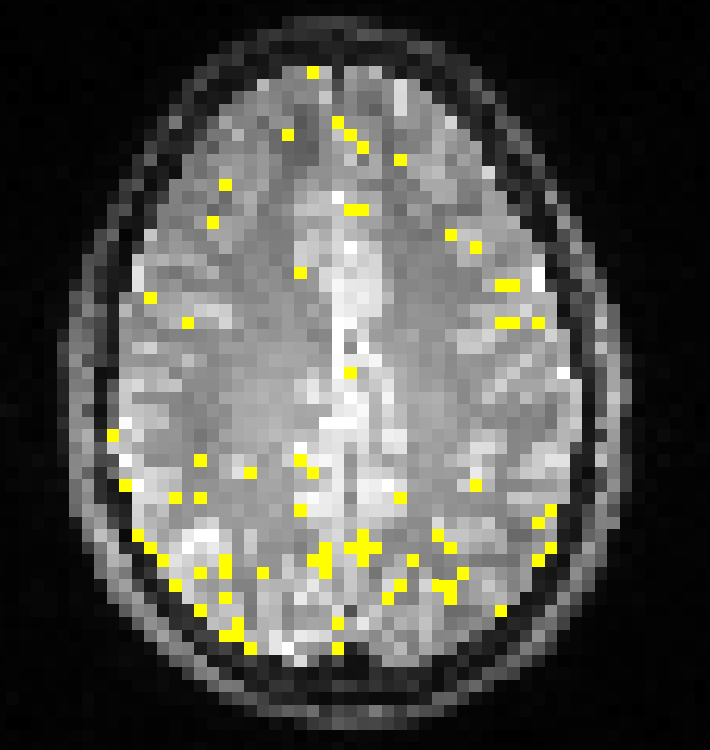
\includegraphics[width=\textwidth]{figures/method1/invivo1/r2}
    \caption{Sub2: correlation map without smoothing.}
    \label{fig:invivo14}
    \end{subfigure}
~
  \begin{subfigure}[t]{0.3\textwidth}
    \centering
    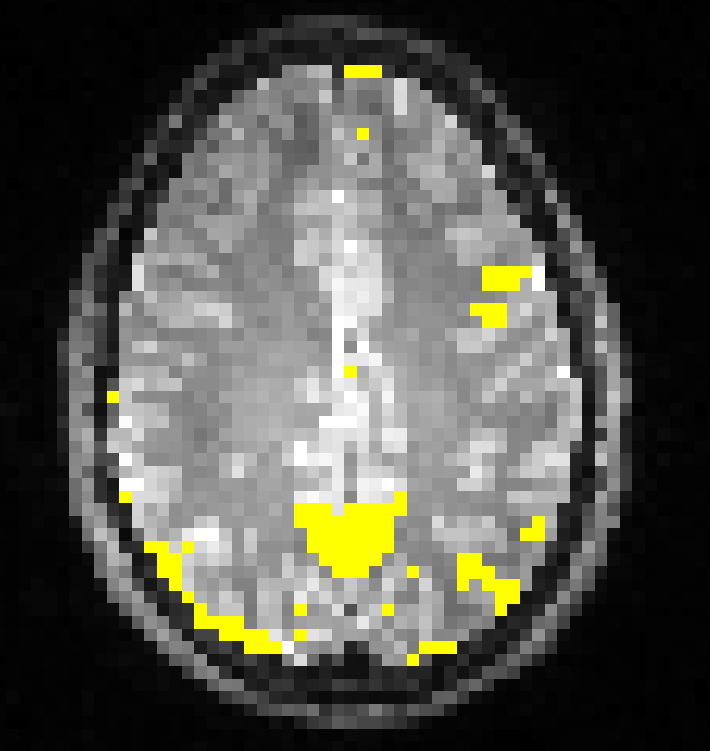
\includegraphics[width=\textwidth]{figures/method1/invivo1/r2_smooth}
    \caption{Sub2: correlation map with smoothing. }
    \label{fig:invivo15}
    \end{subfigure}
~
  \begin{subfigure}[t]{0.3\textwidth}
    \centering
    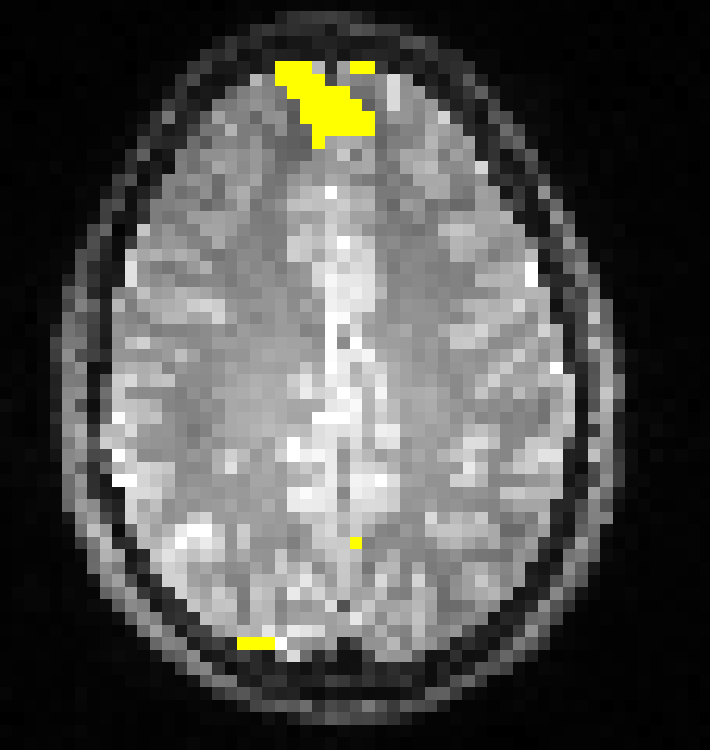
\includegraphics[width=\textwidth]{figures/method1/invivo1/r2_mrf}
    \caption{Sub3: posterior probability by MRF.}
    \label{fig:invivo16}
    \end{subfigure}
    \caption{ Threshold correlation mapand Posterior Connectivity map between
      seed voxel and the current slice, overlaid to T2 image.  (a) Subject 1:
      correlation without smoothing. (b) Subject 1: correlation with
      smoothing. (c) Subject 1: posterior estimated from MRF. (d) Subject 2:
      correlation without smoothing. (e) Correlation without smoothing. (f)
      Posterior estimated from MRF. }
  \label{fig:invivo1}
\end{figure}

\begin{figure}[p] 
  \centering 
  \begin{subfigure}[t]{0.3\textwidth}
    \centering
    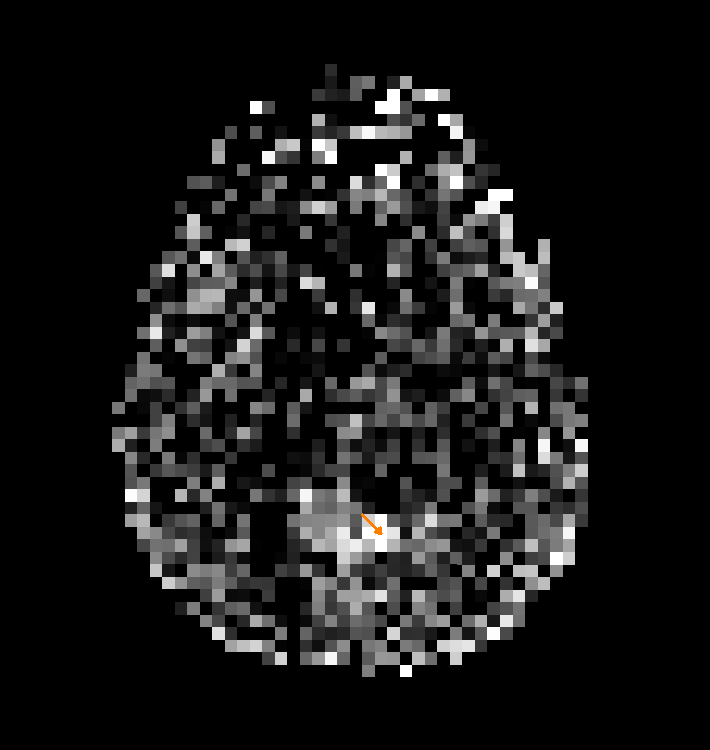
\includegraphics[width=\textwidth]{figures/method1/invivo2/R1_corr_nosmooth}
    \caption{sub1: correlation without smoothing}
    \label{fig:invivo21}
    \end{subfigure}
~
  \begin{subfigure}[t]{0.3\textwidth}
    \centering
    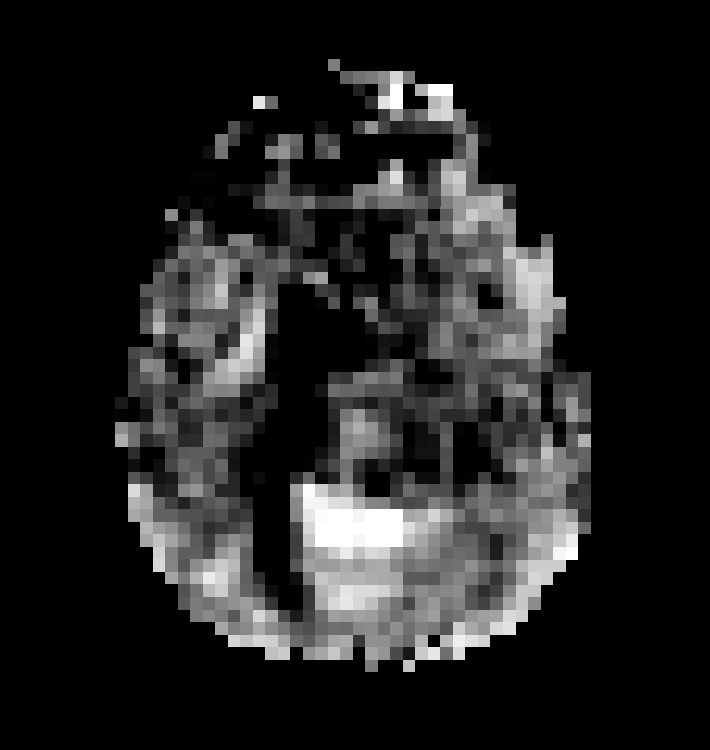
\includegraphics[width=\textwidth]{figures/method1/invivo2/R1_corr_smooth}
    \caption{sub1: Correlation with smoothing}
    \label{fig:invivo22}
    \end{subfigure}
~
  \begin{subfigure}[t]{0.3\textwidth}
    \centering
    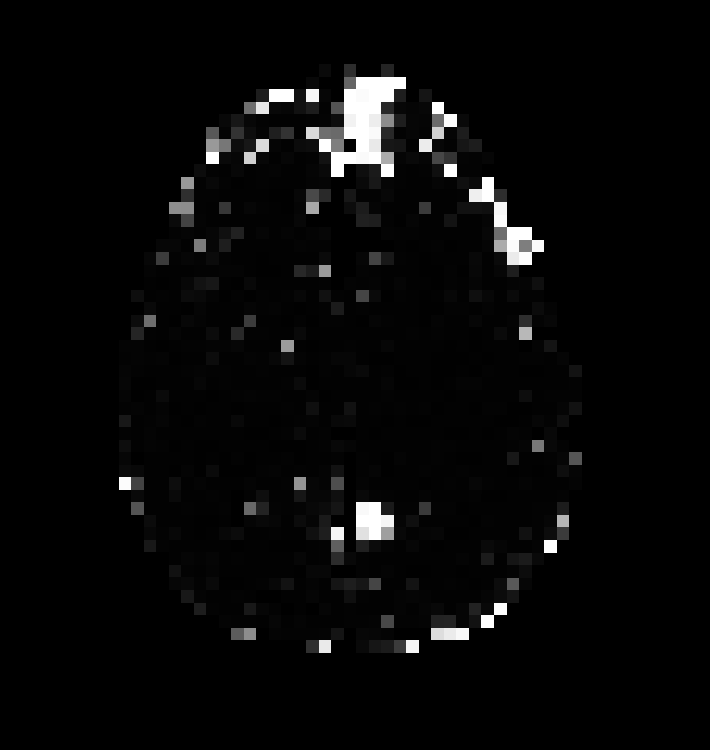
\includegraphics[width=\textwidth]{figures/method1/invivo2/R1_mrf}
    \caption{Posterior from MRF}
    \label{fig:invivo23}
    \end{subfigure}

  \begin{subfigure}[t]{0.3\textwidth}
    \centering
    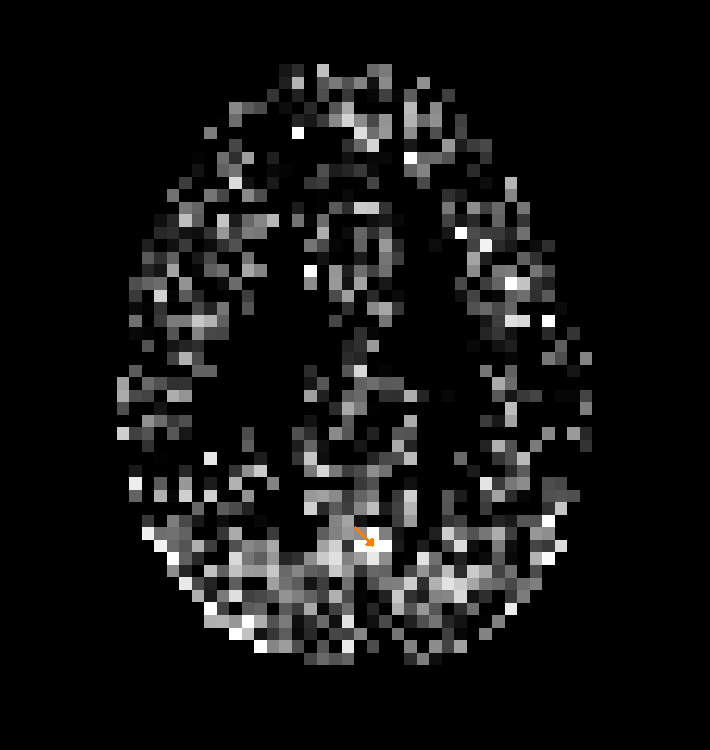
\includegraphics[width=\textwidth]{figures/method1/invivo2/R2_corr_nosmooth}
    \caption{sub2: correlation without smoothing.}
    \label{fig:invivo24}
    \end{subfigure}
~
  \begin{subfigure}[t]{0.3\textwidth}
    \centering
    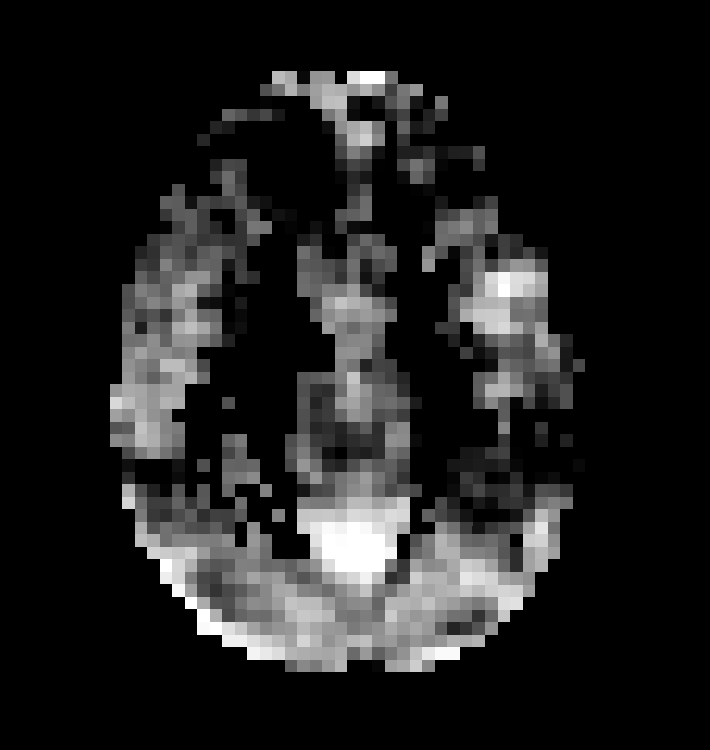
\includegraphics[width=\textwidth]{figures/method1/invivo2/R2_corr_smooth}
    \caption{sub2: correlation with smoothing.}
    \label{fig:invivo25}
    \end{subfigure}
~
  \begin{subfigure}[t]{0.3\textwidth}
    \centering
    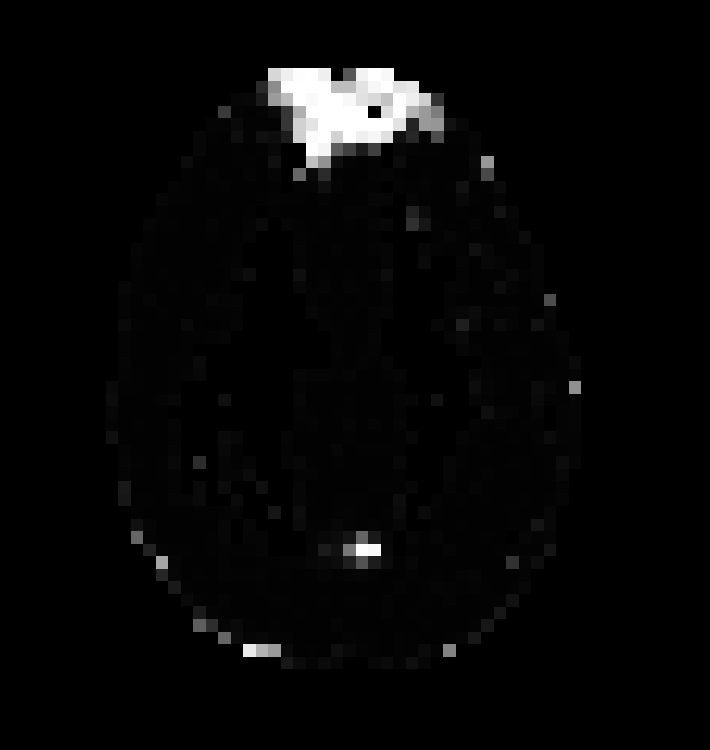
\includegraphics[width=\textwidth]{figures/method1/invivo2/R2_mrf}
    \caption{sub2: posterior from MRF}
    \label{fig:invivo26}
    \end{subfigure}
  \caption{Correlation map and posterior connectivity map between seed voxel and
    slice containing the seed. (a) Subject 1: correlation without
    smoothing. (b) Subject 1: correlation with smoothing. (c) Subject 1:
    posterior estimated from MRF. (d) Subject 2: correlation without
    smoothing. (e) Correlation without smoothing. (f) Posterior estimated
    from MRF. }
  \label{fig:invivo2}
\end{figure}


%%% Local Variables: 
%%% TeX-master: "MyThesis"
%%% End: 
